\subsection{Further Studies on Text Classification Tasks}\label{sec_text}

Our results and simulations are all in the high-dimensional linear regression setting.
How well do they extend to other scenarios?
In this section, we conduct further studies on six text classification datasets.
Our datasets include a movie review sentiment dataset (MR) \cite{pang2005seeing}, a sentence subjectivity dataset (SUBJ) \cite{pang2004sentimental}, a customer reviews dataset (CR) \cite{hu2004mining}, a question type dataset (TREC) \cite{li2002learning}, an opinion polarity dataset (MPQA) \cite{wiebe2005annotating}, and the Stanford sentiment treebank (SST) dataset \cite{socher2013recursive}.
Our model consists of a word embedding layer with GloVe embeddings \cite{pennington2014glove} followed by a long-short term memory (LSTM) or a multi-layer perception (MLP) layer \cite{lei2018simple}.\footnote{For MLP, we apply an average pooling layer over word embeddings. For LSTM, we add a shared feature representation layer on top of word embeddings.}


\paragraph{Sample size ratio.}
First, we show that our observation in Figure \ref{fig_size} also occurs in the text classification tasks.
In Figure \ref{fig_ab_data}, we observe that for multiple example task pairs, increasing task one's sample size improves task two's prediction accuracy initially but hurts eventually.
On the $y$-axis, we plot task two's test accuracy using HPS, subtracted by its STL test accuracy.
We fix task two's sample size at $1000$ and increase task one's sample size from $100$ to $3000$.

These examples and Figure \ref{fig_size} suggest a natural progressive training schedule, where we add samples progressively until performance drops.
Concretely, here is one implementation of this idea.
\begin{itemize}
	\item We divide the training data into $S$ batches.
	We divide the training procedure into $S$ stages. During every stage, we progressively add one more data batch.
	\item During every stage, we train for $T$ epochs using only the $S$ batches. If the validation accuracy drops compared to the previous round's result or reaches the desired threshold $\tau$, we terminate.
\end{itemize}
If we apply this procedure to the settings of Figure \ref{fig_ab_data} and \ref{fig_size}, it will terminate once reaching the optimal sample ratio.
The advantage of this procedure is that it reduces the computational cost compared to standard round-robin training schedules.
For example, if the process terminates at 30\% of all batches, then SGD only passes over 30\% of its data, whereas standard round-robin training passes over 100\% of task one's data.


We evaluate the progressive training procedure on the six text classification datasets.
First, we conduct multi-task training over all the $15$ two-task pairs from the six datasets.
We focus on task two's test accuracy and set $\tau$ as task two's test accuracy obtained via the standard round-robin training schedule.
We include all of task two's data and progressively add task one's data using the procedure described above.
Since the prediction accuracy has been controlled the same, we compare the computational cost.
We find that when averaged over all the $15$ two-task pairs, this procedure requires only $45\%$ of the computational cost to reach the desired accuracy $\tau$ for task two.
Second, we conduct multi-task training on all six datasets jointly.
We extend our procedure to all six datasets. We include the data from all tasks except SST. For SST, we progressively add data similar to the above procedure.
We set $\tau$ to be the average test accuracy of all the six tasks obtained using standard round-robin training.
We find that adding samples progressively from SST requires less than $35\%$ of the computational cost to reach the same average test accuracy $\tau$.







\paragraph{Covariate shift.}
Recall from Example \ref{ex_covshift} that having covariate shifts worsens the variance (hence the loss) of hard parameter sharing when the sample ratio increases.
This highlights the need for correcting covariate shifts when the sample size ratio rises.
To this end, we study a covariance alignment procedure proposed in \citet{WZR20}, designed to correct covariate shifts.
The idea is to add an alignment module between the input and the shared module $B$.
This module is then trained together with $B$ and the output layers. We refer to \citet{WZR20} for more details about the procedure and the implementation.

We conduct multi-task training on all $15$ task pairs from the six datasets.
In Figure \ref{fig_ab_cov}, we measure the performance gains from performing covariance alignment vs. HPS.
To get a robust comparison, we average the improvements over the 15 task pairs.
The result shows that as the sample size ratio increases, performing covariance alignment provides more significant gains over HPS.
We fix task two's sample size at $1,000$, and increase task one's sample size from $1,000$ to $3,000$.





\begin{figure}%
	\begin{subfigure}[t]{0.5\textwidth}
		\centering
		\vspace{0pt}
		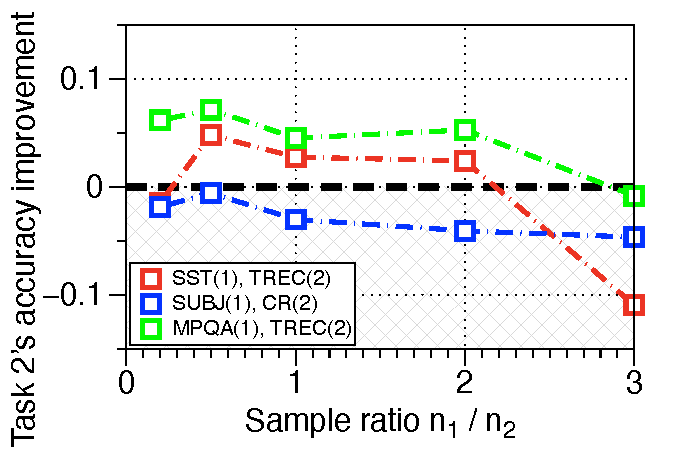
\includegraphics[width=0.8\textwidth]{figures/fig3a.pdf}
		\caption{HPS vs. STL}
		\label{fig_ab_data}
	\end{subfigure}\hfill
	\begin{subfigure}[t]{0.5\textwidth}
		\centering
		\vspace{0pt}
		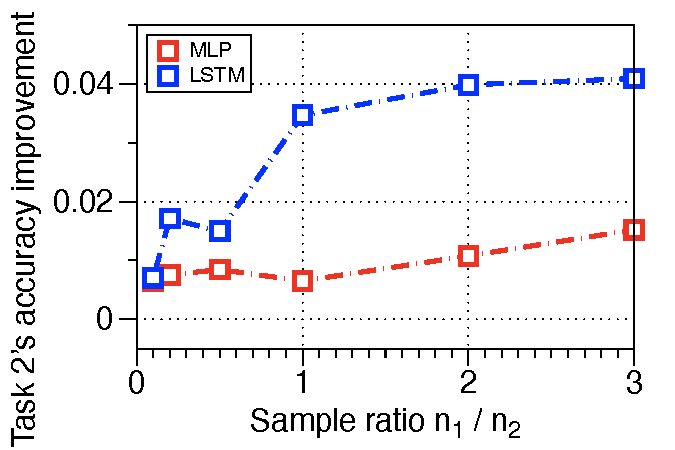
\includegraphics[width=0.8\textwidth]{figures/fig3b.pdf}
		\caption{HPS vs. covariance alignment}
		\label{fig_ab_cov}
	\end{subfigure}
	\caption{Comparing hard parameter sharing (HPS) to single-task learning (STL) and a covariance alignment approach proposed by \citet{WZR20}:
	In Figure \ref{fig_ab_data}, we observe that for multiple task pairs, increasing task one's sample size improves task two's prediction accuracy initially, but hurts eventually -- a phenomenon similar  to Figure \ref{fig_size}.
	In Figure \ref{fig_ab_cov}, we observe that as task one's sample size increases, covariance alignment improves more over HPS.}
	\label{fig_text}
\end{figure}

